%!TEX program = xelatex
%!TEX root = ../all_beamer.tex


%\documentclass[aspectratio=169,10pt]{beamer}
%
%% ─── Theme & Colours ───────────────────────────────────────────────────────────
%% !TEX root = all_beamer.tex
% ==============================================================================
% HEADER LATEX PER PRESENTAZIONI BEAMER
% Corso di Machine Learning - Giorgio Gambosi
% Università di Roma "Tor Vergata"
% ==============================================================================

% ------------------------------------------------------------------------------
% CLASSE DOCUMENTO E METADATI
% ------------------------------------------------------------------------------
\documentclass[aspectratio=169, 10pt]{beamer}

\subtitle{Course of Machine Learning}
\author{Giorgio Gambosi}
\institute[Tor Vergata]{Master's Degree in Computer Science\\University of Rome ``Tor Vergata''}
\date{A.Y. 2025--2026}

% ------------------------------------------------------------------------------
% PACCHETTI MATEMATICI
% ------------------------------------------------------------------------------
\usepackage{amsmath, amssymb, amsfonts, mathtools, amsthm}
\usepackage{bm}              % Simboli matematici in grassetto
\usepackage{upgreek}         % Lettere greche dritte
\usepackage{derivative}      % Gestione semplificata delle derivate

% ------------------------------------------------------------------------------
% PACCHETTI GRAFICI E VISUALIZZAZIONE
% ------------------------------------------------------------------------------
\usepackage{graphicx}        % Inclusione immagini
\usepackage{xcolor}          % Gestione colori
\usepackage{xkcdcolors}      % Colori aggiuntivi stile xkcd
\usepackage{microtype}       % Miglioramenti tipografici

% ------------------------------------------------------------------------------
% PACCHETTI PER TABELLE
% ------------------------------------------------------------------------------
\usepackage{booktabs}        % Tabelle professionali
\usepackage{array}           % Estensioni per tabelle
\usepackage{multirow}        % Celle multi-riga
\usepackage{multicol}        % Layout multi-colonna

% ------------------------------------------------------------------------------
% TIKZ E PGFPLOTS
% ------------------------------------------------------------------------------
\usepackage{tikz}
\usepackage{tikz-network}
\usepackage[customcolors]{hf-tikz}
\usepackage{pgfplots}
\pgfplotsset{compat=1.18}
\usepgfplotslibrary{fillbetween}

% Librerie TikZ
\usetikzlibrary{arrows, arrows.meta, decorations.pathmorphing, decorations.pathreplacing}
\usetikzlibrary{decorations.markings, snakes, positioning, backgrounds, fit, shadows}
\usetikzlibrary{automata, patterns, calc, intersections, through, shapes}
\usetikzlibrary{shapes.geometric, shapes.arrows, scopes, chains, matrix}

% ------------------------------------------------------------------------------
% ALTRI PACCHETTI
% ------------------------------------------------------------------------------
\usepackage[skins]{tcolorbox}  % Box colorati
\usepackage{subcaption}         % Sottocaption per figure
\usepackage{listings}           % Inclusione codice sorgente

% ------------------------------------------------------------------------------
% TEMA E STILE BEAMER
% ------------------------------------------------------------------------------
\usetheme{Madrid}
\usecolortheme{whale}
\useinnertheme{rounded}
\usefonttheme{professionalfonts}
\setbeamertemplate{navigation symbols}{}  % Rimuove simboli di navigazione

% ------------------------------------------------------------------------------
% DEFINIZIONE COLORI PERSONALIZZATI
% ------------------------------------------------------------------------------
% Colori principali del tema
\definecolor{MainBlue}{RGB}{31,56,100}      % Blu principale (header, titoli)
\definecolor{AccentBlue}{RGB}{70,130,180}   % Blu accento (blocchi)
\definecolor{AlertRed}{RGB}{160,30,30}      % Rosso per alert
\definecolor{ExGreen}{RGB}{30,120,60}       % Verde per esempi
\definecolor{BlockBg}{RGB}{220,232,246}     % Sfondo blocchi
\definecolor{torgray}{RGB}{220,225,235}     % Grigio Tor Vergata

% Colori alternativi (Tor Vergata style)
\definecolor{TvDark}{RGB}{30,50,80}         % Blu scuro header
\definecolor{TvMid}{RGB}{70,100,140}        % Blu medio blocchi
\definecolor{TvLight}{RGB}{210,220,235}     % Blu chiaro sfondi
\definecolor{TvAlert}{RGB}{160,30,30}       % Rosso alert
\definecolor{TvGreen}{RGB}{20,100,50}       % Verde esempi

% Colori supplementari
\definecolor{torred}{RGB}{153,0,0}
\definecolor{torcyan}{RGB}{0,112,192}
\definecolor{cerise}{HTML}{DA3A62}
\definecolor{teal}{HTML}{029386}
\definecolor{slateblue}{HTML}{5B5EA6}
\definecolor{orange}{HTML}{F97306}

% Colori per nodi TikZ
\definecolor{nodeblue}{RGB}{101,140,196}    % xkcd Faded Blue

% ------------------------------------------------------------------------------
% CONFIGURAZIONE COLORI BEAMER
% ------------------------------------------------------------------------------
\setbeamercolor{frametitle}{bg=MainBlue, fg=white}
\setbeamercolor{title}{bg=MainBlue, fg=white}
\setbeamercolor{structure}{fg=MainBlue}

% Blocchi standard
\setbeamercolor{block title}{bg=AccentBlue, fg=white}
\setbeamercolor{block body}{bg=BlockBg}

% Blocchi alert
\setbeamercolor{block title alerted}{bg=AlertRed, fg=white}
\setbeamercolor{block body alerted}{bg=red!8}

% Blocchi esempio
\setbeamercolor{block title example}{bg=ExGreen, fg=white}
\setbeamercolor{block body example}{bg=green!7}

% ------------------------------------------------------------------------------
% CONFIGURAZIONE FONT BEAMER
% ------------------------------------------------------------------------------
\setbeamerfont{frametitle}{size=\normalsize,series=\bfseries}
\setbeamerfont{block title}{size=\small,series=\bfseries}

% ------------------------------------------------------------------------------
% STILI TIKZ PERSONALIZZATI
% ------------------------------------------------------------------------------
\tikzset{
  >=latex,  % Frecce stile LaTeX di default
  % Nodi per reti neurali
  node/.style={thick,circle,draw=myblue,minimum size=22,inner sep=0.5,outer sep=0.6},
  node in/.style={node,green!20!black,draw=mygreen!30!black,fill=mygreen!25},
  node hidden/.style={node,blue!20!black,draw=myblue!30!black,fill=myblue!20},
  node convol/.style={node,orange!20!black,draw=myorange!30!black,fill=myorange!20},
  node out/.style={node,red!20!black,draw=myred!30!black,fill=myred!20},
  % Connessioni
  connect/.style={thick,mydarkblue},
  connect arrow/.style={-{Latex[length=4,width=3.5]},thick,mydarkblue,shorten <=0.5,shorten >=1},
  % Stili numerati per facile mappatura
  node 1/.style={node in},
  node 2/.style={node hidden},
  node 3/.style={node out}
}

% ------------------------------------------------------------------------------
% AMBIENTI TEOREMI
% ------------------------------------------------------------------------------
\setbeamertemplate{theorems}[numbered]
\newtheorem{mytheorem}{Theorem}
\newtheorem{mydefinition}{Definition}

% ------------------------------------------------------------------------------
% CONFIGURAZIONE LISTINGS (CODICE)
% ------------------------------------------------------------------------------
\lstset{
  language=Python,
  basicstyle=\ttfamily\tiny,
  keywordstyle=\color{MainBlue}\bfseries,
  commentstyle=\color{gray},
  frame=single,
  breaklines=true,
}

% ==============================================================================
% MACRO MATEMATICHE PERSONALIZZATE
% ==============================================================================

% ------------------------------------------------------------------------------
% SPAZI CALLIGRAFICI (Calligraphic spaces)
% ------------------------------------------------------------------------------
\providecommand{\calX}{\mathcal{X}}         % Spazio input
\providecommand{\calY}{\mathcal{Y}}         % Spazio output
\providecommand{\calH}{\mathcal{H}}         % Spazio ipotesi
\providecommand{\calT}{\mathcal{T}}         % Training set
\providecommand{\calA}{\mathcal{A}}         % Algoritmo
\providecommand{\calR}{\mathcal{R}}         % Rischio
\providecommand{\calF}{\mathcal{F}}         % Famiglia di funzioni
\providecommand{\calL}{\mathcal{L}}         % Loss function

% Alias per compatibilità
\providecommand{\Rr}{\mathcal{R}}
\providecommand{\Tr}{\mathcal{T}}
\providecommand{\Hr}{\mathcal{H}}

% ------------------------------------------------------------------------------
% RISCHIO E PROBABILITÀ
% ------------------------------------------------------------------------------
\providecommand{\barR}{\overline{\mathcal{R}}}  % Rischio empirico
\providecommand{\EmpR}{\overline{\mathcal{R}}}  % Rischio empirico (alias)
\providecommand{\Rbar}{\overline{\mathcal{R}}}  % Rischio empirico (alias)
\providecommand{\pM}{p_M}                       % Probabilità modello
\providecommand{\pC}{p_C}                       % Probabilità corretta
\providecommand{\Prob}[2]{\mathbb{P}_{#1}\!\left[#2\right]}  % Probabilità

% ------------------------------------------------------------------------------
% FUNZIONI INDICATRICI
% ------------------------------------------------------------------------------
\providecommand{\indicator}[1]{\mathbf{1}\!\left[#1\right]}  % Funzione indicatrice
\providecommand{\ind}[1]{\mathbf{1}[#1]}                      % Versione breve

% ------------------------------------------------------------------------------
% OPERATORI MATEMATICI
% ------------------------------------------------------------------------------
\providecommand{\argmax}{\operatorname*{arg\,max}}  % Argomento del massimo
\providecommand{\argmin}{\operatorname*{arg\,min}}  % Argomento del minimo
\providecommand{\vcd}[1]{\operatorname{VCdim}(#1)} % VC dimension
\providecommand{\defeq}{\stackrel{\text{def}}{=}}  % Definito come

% ------------------------------------------------------------------------------
% VETTORI E MATRICI (Bold Math)
% ------------------------------------------------------------------------------
% Vettori minuscoli
\providecommand{\bx}{\mathbf{x}}            % Vettore x
\providecommand{\bz}{\mathbf{z}}            % Vettore z
\providecommand{\bw}{\mathbf{w}}            % Vettore peso
\providecommand{\btt}{\mathbf{t}}           % Vettore target
\providecommand{\wvec}{\mathbf{w}}          % Vettore peso (alias)
\providecommand{\bth}{\boldsymbol{\theta}}  % Parametro theta

% Matrici maiuscole
\providecommand{\bX}{\mathbf{X}}            % Matrice dati
\providecommand{\bZ}{\mathbf{Z}}            % Matrice Z
\providecommand{\Xmat}{\mathbf{X}}          % Matrice dati (alias)
\providecommand{\Hmat}{\mathbf{H}}          % Matrice H
\providecommand{\Smat}{\mathbf{S}}          % Matrice scatter generica
\providecommand{\bS}{\mathbf{S}}            % Matrice scatter
\providecommand{\Ii}{\mathbf{I}}            % Matrice identità
\providecommand{\bZero}{\mathbf{0}}         % Vettore zero
\providecommand{\bPsi}{\boldsymbol{\Psi}}   % Matrice Psi

% Medie (overline)
\providecommand{\ox}{\overline{\mathbf{x}}} % Media vettore x
\providecommand{\ow}{\overline{\mathbf{w}}} % Media vettore w
\providecommand{\oX}{\overline{\mathbf{X}}} % Media matrice X

% Matrici scatter specifiche (analisi discriminante)
\providecommand{\SW}{\mathbf{S}_W}          % Within-class scatter
\providecommand{\SB}{\mathbf{S}_B}          % Between-class scatter
\providecommand{\ST}{\mathbf{S}_T}          % Total scatter
\providecommand{\GX}{G_{\mathbf{X}}}        % Matrice Gram

% ------------------------------------------------------------------------------
% COMANDI DI FORMATTAZIONE TESTO
% ------------------------------------------------------------------------------
\providecommand{\term}[1]{\textbf{\color{accent}#1}}        % Termine importante
\providecommand{\halert}[1]{{\color{AlertRed}\textbf{#1}}}  % Alert rosso
\providecommand{\mlalert}[1]{{\color{AccentBlue}\textbf{#1}}}  % Alert blu
\providecommand{\mlemph}[1]{{\color{MainBlue}\textit{#1}}}  % Enfasi blu

% ==============================================================================
% FINE HEADER
% ==============================================================================

\newcommand{\blankpage}{
\clearpage
\thispagestyle{empty}
\null
\clearpage
}

%\usetheme{default}
%\usecolortheme{default}
%


%\definecolor{mllightgray}{RGB}{245,245,245}
%\definecolor{mldarkbg}{RGB}{18,32,58}
%
%\setbeamercolor{frametitle}{fg=white,bg=MainBlue}
%\setbeamercolor{title}{fg=white}
%\setbeamercolor{subtitle}{fg=AlertRed}
%\setbeamercolor{author}{fg=white}
%\setbeamercolor{date}{fg=white!80}
%\setbeamercolor{institute}{fg=white!80}
%\setbeamercolor{normal text}{fg=black}
%\setbeamercolor{item}{fg=MainBlue}
%\setbeamercolor{subitem}{fg=AccentBlue}
%\setbeamercolor{block title}{bg=MainBlue,fg=white}
%\setbeamercolor{block body}{bg=mllightgray,fg=black}
%\setbeamercolor{alerted text}{fg=AccentBlue}
%\setbeamercolor{structure}{fg=MainBlue}
%\setbeamercolor{section in head/foot}{bg=mldarkbg,fg=white}
%\setbeamercolor{footline}{bg=mldarkbg,fg=white!70}
%% Linear Classification – Beamer Presentation
%% Based on notes by Giorgio Gambosi, University of Rome "Tor Vergata"
%% Style modelled on ml-nonparam-regr-beamer.pdf

%\documentclass[aspectratio=169]{beamer}



% ─── Fonts ─────────────────────────────────────────────────────────────────────
%\usepackage[T1]{fontenc}
%\usefonttheme{professionalfonts}
%\setbeamerfont{frametitle}{size=\large,series=\bfseries}
%\setbeamerfont{title}{size=\LARGE,series=\bfseries}
%\setbeamerfont{subtitle}{size=\large}
%\setbeamerfont{block title}{series=\bfseries}

% ─── Packages ──────────────────────────────────────────────────────────────────
%\usepackage{amsmath,amssymb,bm}
%\usepackage{mathtools}
%\usepackage{graphicx}
%\usepackage{xcolor}
%\usepackage{booktabs}
%\usepackage{tikz}
%\usetikzlibrary{arrows.meta,shapes.geometric,positioning,calc,decorations.pathreplacing}

% ─── Header / Footer ───────────────────────────────────────────────────────────
%\setbeamertemplate{navigation symbols}{}
%\setbeamertemplate{footline}{%
%  \leavevmode%
%  \hbox{%
%    \begin{beamercolorbox}[wd=.33\paperwidth,ht=2.4ex,dp=1ex,leftskip=4pt]{footline}%
%      \footnotesize G.~Gambosi
%    \end{beamercolorbox}%
%    \begin{beamercolorbox}[wd=.34\paperwidth,ht=2.4ex,dp=1ex,center]{footline}%
%      \footnotesize Notes on Machine Learning
%    \end{beamercolorbox}%
%    \begin{beamercolorbox}[wd=.33\paperwidth,ht=2.4ex,dp=1ex,right,rightskip=4pt]{footline}%
%      \footnotesize \insertframenumber{} / \inserttotalframenumber
%    \end{beamercolorbox}%
%  }%
%}
%
%\setbeamertemplate{frametitle}{%
%  \nointerlineskip%
%  \begin{beamercolorbox}[wd=\paperwidth,ht=2.6ex,dp=1ex,leftskip=8pt,rightskip=8pt]{frametitle}%
%    \usebeamerfont{frametitle}\insertframetitle%
%    \ifx\insertframesubtitle\empty\else%
%      \hfill{\footnotesize\color{white!80}\insertframesubtitle}%
%    \fi%
%  \end{beamercolorbox}%
%}
%
%\setbeamertemplate{itemize item}{\scriptsize\raise1.5pt\hbox{\textbullet}}
%\setbeamertemplate{itemize subitem}{\scriptsize\raise1.5pt\hbox{$\circ$}}
%\setbeamertemplate{itemize subsubitem}{\tiny\raise1.5pt\hbox{$\diamond$}}
%
% ─── Macros ────────────────────────────────────────────────────────────────────

%\newcommand{\t}{\mathbf{t}}
%\newcommand{\ow}{\overline{\mathbf{w}}}
%\newcommand{\ox}{\overline{\mathbf{x}}}
%\newcommand{\oX}{\overline{\mathbf{X}}}
%
%%\newcommand{\y}{\mathbf{y}}
%%\newcommand{\Y}{\mathbf{Y}}
%%\newcommand{\VSigma}{\boldsymbol{\Sigma}}
%%\newcommand{\Vmu}{\boldsymbol{\mu}}
%%\newcommand{\Vtheta}{\boldsymbol{\theta}}
%%\newcommand{\VPsi}{\boldsymbol{\Psi}}
%%\newcommand{\Zero}{\mathbf{0}}
%%\newcommand{\A}{\mathbf{A}}
%\newcommand{\Hmat}{\mathbf{H}}
%%\newcommand{\I}{\mathbf{I}}
%
%\newcommand{\mlalert}[1]{{\color{AccentBlue}\textbf{#1}}}
%\newcommand{\mlemph}[1]{{\color{MainBlue}\textit{#1}}}

% ─── Title page background ─────────────────────────────────────────────────────

% ─── Document ──────────────────────────────────────────────────────────────────
\title{Discriminative Probabilistic Classification}
%\subtitle{Course of Machine Learning}
%\author{Giorgio Gambosi}
%\institute{Master Degree in Computer Science\\University of Rome ``Tor Vergata''}
%\date{Academic Year 2025--2026}
%
%\begin{document}

%% ══════════════════════════════════════════════════════════════════
%% TITLE
%% ══════════════════════════════════════════════════════════════════
\begin{frame}
  \titlepage
\end{frame}

%% ══════════════════════════════════════════════════════════════════
%% TABLE OF CONTENTS
%% ══════════════════════════════════════════════════════════════════
\begin{frame}{Outline}
  \tableofcontents
\end{frame}

%% ══════════════════════════════════════════════════════════════════
\section{Generalized Linear Models}
%% ══════════════════════════════════════════════════════════════════
%\sectionslide{Generalized Linear Models}{A unifying framework for regression and classification}

\begin{frame}{Motivation}
  \begin{itemize}
    \item In classification and regression, posterior class probabilities $p(C_k|\x)$ often take the form of a \mlalert{sigmoid} (binary) or \mlalert{softmax} (multiclass).
    \item These arguments are linear combinations of input features.
    \item This pattern is not accidental: it reflects the framework of \mlalert{Generalized Linear Models (GLMs)}.
  \end{itemize}
  \vspace{0.3cm}
  \begin{block}{Key insight}
    GLMs provide a unifying language connecting \emph{linear predictors}, \emph{probabilistic modeling}, and \emph{nonlinear response functions}.
  \end{block}
\end{frame}

\begin{frame}{Definition of a GLM}
  A \mlalert{Generalized Linear Model} is a function of the form:
  \[
    h(\x) = f\!\left(\ow^T\ox\right)
  \]
  where:
  \begin{itemize}
    \item $\ox = (1, \x^T)^T$ is the \mlemph{augmented feature vector}.
    \item $\ow = (b, \w^T)^T$ is the \mlemph{parameter vector} (including bias).
    \item $f$ is the \mlalert{response function} (or \emph{link function}): a generally nonlinear map from $\mathbb{R}$ to the appropriate output range.
  \end{itemize}
  \vspace{0.3cm}
  \begin{block}{Role of $f$}
    \begin{itemize}
      \item Maps the linear predictor $\ow^T\ox \in \mathbb{R}$ to a meaningful output range (e.g.\ $(0,1)$ for probabilities).
      \item Despite the nonlinearity, GLMs retain \mlalert{linear iso-surfaces} (hyperplane decision boundaries).
    \end{itemize}
  \end{block}
\end{frame}

\begin{frame}{Linear Decision Boundaries}
  \begin{columns}[T]
    \begin{column}{0.6\textwidth}
      Consider the iso-surface $h(\x) = c$. Then:
      \[
        f(\ow^T\ox) = c \;\Rightarrow\; \ow^T\ox = f^{-1}(c) = c'
      \]
      \begin{itemize}
        \item This defines a \mlalert{hyperplane} in feature space.
        \item All iso-surfaces of a GLM are hyperplanes.
        \item Decision boundaries are linear in the input space.
      \end{itemize}
    \end{column}
    \begin{column}{0.36\textwidth}
      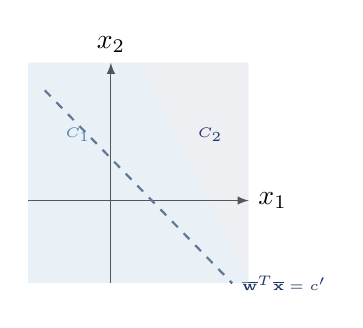
\begin{tikzpicture}[scale=0.7]
        \draw[->] (-1.5,0)--(2.5,0) node[right]{$x_1$};
        \draw[->] (0,-1.5)--(0,2.5) node[above]{$x_2$};
        \draw[MainBlue,thick,dashed] (-1.2,2)--(2.2,-1.5) node[right,font=\tiny]{$\ow^T\ox=c'$};
        \fill[AccentBlue!30,opacity=0.4] (-1.5,2.5) -- (0.5,2.5) -- (2.5,-1.5) -- (-1.5,-1.5) -- cycle;
        \fill[MainBlue!20,opacity=0.4] (0.5,2.5) -- (2.5,2.5) -- (2.5,-1.5) -- cycle;
        \node[AccentBlue,font=\tiny] at (-0.6,1.2) {$C_1$};
        \node[MainBlue,font=\tiny] at (1.8,1.2) {$C_2$};
      \end{tikzpicture}
    \end{column}
  \end{columns}
\end{frame}

%% ── Exponential Families ──
\subsection{Exponential Families}

\begin{frame}{Exponential Family Distributions}
  A GLM arises when the conditional distribution $p(t|\x)$ belongs to the \mlalert{exponential family}:
  \[
    p(t|\x) = \frac{1}{s}\,g(\Vtheta(\x))\,f\!\left(\frac{t}{s}\right)
    \exp\!\left(\frac{1}{s}\Vtheta(\x)^T\mathbf{u}(t)\right)
  \]
  \begin{itemize}
    \item $\Vtheta(\x)$ is the \mlalert{natural parameter}.
    \item $\mathbf{u}(t)$ are the \mlalert{sufficient statistics}.
    \item $s$ is a scale parameter.
    \item Includes: Normal, Bernoulli, Categorical, Poisson, Exponential, \ldots
  \end{itemize}
  \vspace{0.2cm}
  \begin{block}{Three GLM conditions}
    \begin{enumerate}
      \item $p(t|\x)$ belongs to the exponential family.
      \item Prediction targets $\mathbb{E}[\mathbf{u}(t)|\x]$.
      \item The natural parameter is linear: $\Vtheta(\x) = \ow^T\ox$.
    \end{enumerate}
  \end{block}
\end{frame}

\begin{frame}{GLM with Normal Distribution}
  \begin{columns}[T]
    \begin{column}{0.55\textwidth}
      \textbf{Setting:} $t \in \mathbb{R}$, $p(t|\x) = \mathcal{N}(t;\mu(\x),\sigma^2)$.\\[0.4em]
      \textbf{Exponential-family identification:}
      \[
        \mathbf{u}(t) = \begin{pmatrix}t \\ t^2\end{pmatrix},\quad
        \Vtheta(\x) = \begin{pmatrix}\mu(\x)/\sigma^2 \\ -1/(2\sigma^2)\end{pmatrix}
      \]
      \textbf{Prediction target:} $\mathbb{E}[t|\x] = \mu(\x)$.\\[0.4em]
      \textbf{GLM predictor:}
      \[
        h(\x) = \sigma^2\,\ow^T\ox
      \]
    \end{column}
    \begin{column}{0.42\textwidth}
      \begin{block}{Result}
        Ordinary \mlalert{linear regression} is the GLM corresponding to the \emph{Normal distribution} with the \emph{identity link function}.
      \end{block}
      \vspace{0.3em}
      \begin{itemize}
        \item Response function: $f = \text{identity}$.
        \item Variance $\sigma^2$ assumed fixed.
      \end{itemize}
    \end{column}
  \end{columns}
\end{frame}

\begin{frame}{GLM with Bernoulli Distribution}
  \begin{columns}[T]
    \begin{column}{0.55\textwidth}
      \textbf{Setting:} $t \in \{0,1\}$, $p(t|\x) = \pi(\x)^t(1-\pi(\x))^{1-t}$.\\[0.4em]
      \textbf{Sufficient statistic:} $\mathbf{u}(t) = t$.\\[0.4em]
      \textbf{Natural parameter (log-odds):}
      \[
        \theta(\x) = \log\frac{\pi(\x)}{1-\pi(\x)}
      \]
      \textbf{Response (inverse link):}
      \[
        h(\x) = \pi(\x) = \frac{1}{1+e^{-\theta(\x)}}
      \]
    \end{column}
    \begin{column}{0.42\textwidth}
      \begin{block}{Result}
        Assuming $\theta(\x) = \ow^T\ox$ yields \mlalert{logistic regression}:
        \[
          h(\x) = \frac{1}{1+e^{-\ow^T\ox}}
        \]
      \end{block}
      \begin{itemize}
        \item Sigmoid maps $\mathbb{R} \to (0,1)$.
        \item Natural consequence of the Bernoulli + GLM combination.
      \end{itemize}
    \end{column}
  \end{columns}
\end{frame}

\begin{frame}{GLM with Categorical Distribution}
  \textbf{Setting:} $t \in \{1,\ldots,K\}$, one-hot encoding $(t_1,\ldots,t_K)$.
  \[
    p(t|\x) = \prod_{i=1}^K \pi_i(\x)^{t_i}, \quad \sum_{i=1}^K\pi_i(\x) = 1.
  \]
  \begin{columns}[T]
    \begin{column}{0.5\textwidth}
      \textbf{Natural parameters (log-odds vs.\ class $K$):}
      \[
        \theta_i(\x) = \log\frac{\pi_i(\x)}{\pi_K(\x)}
      \]
      \textbf{Assuming} $\theta_i(\x) = \ow_i^T\ox$:
    \end{column}
    \begin{column}{0.47\textwidth}
      \textbf{Response (\mlalert{softmax}):}
      \[
        h_i(\x) = \pi_i(\x) = \frac{e^{\ow_i^T\ox}}{\sum_{j=1}^K e^{\ow_j^T\ox}}
      \]
    \end{column}
  \end{columns}
  \vspace{0.3cm}
  \begin{block}{Result}
    \mlalert{Softmax regression} is the GLM for categorical outcomes. Each class has a linear discriminant function; the softmax ensures a valid probability distribution.
  \end{block}
\end{frame}

\begin{frame}{Further GLM Examples}
  \begin{columns}[T]
    \begin{column}{0.48\textwidth}
      \begin{block}{Poisson Regression}
        \begin{itemize}
          \item $t \in \{0,1,\ldots\}$ (count data).
          \item $p(t|\x) = \frac{\lambda(\x)^t}{t!}e^{-\lambda(\x)}$.
          \item Natural parameter: $\theta(\x) = \log\lambda(\x)$.
          \item Predictor: $h(\x) = e^{\ow^T\ox}$.
          \item \textit{Exponential link ensures positive mean.}
        \end{itemize}
      \end{block}
    \end{column}
    \begin{column}{0.48\textwidth}
      \begin{block}{Exponential Regression}
        \begin{itemize}
          \item $t \in [0,\infty)$ (waiting times).
          \item $p(t|\x) = \lambda(\x)e^{-\lambda(\x)t}$.
          \item Natural parameter: $\theta(\x) = -\lambda(\x)$.
          \item Predictor: $h(\x) = -1/(\ow^T\ox)$.
          \item \textit{Inverse link; requires $\ow^T\ox < 0$.}
        \end{itemize}
      \end{block}
    \end{column}
  \end{columns}
  \vspace{0.3cm}
  \begin{itemize}
    \item GLMs offer a \mlalert{coherent and unifying framework}: many classical methods emerge as special cases.
    \item The response function is \emph{determined} by the choice of distribution — not chosen arbitrarily.
  \end{itemize}
\end{frame}

%% ══════════════════════════════════════════════════════════════════
\section{Discriminative Approach}
%% ══════════════════════════════════════════════════════════════════
%\sectionslide{Discriminative Approach}{Modeling posteriors directly, without the joint distribution}

\begin{frame}{Discriminative vs.\ Generative}
  \begin{columns}[T]
    \begin{column}{0.48\textwidth}
      \begin{block}{Generative approach}
        \begin{itemize}
          \item Models $p(\x|C_k)$ and $p(C_k)$.
          \item Applies Bayes' rule to compute $p(C_k|\x)$.
          \item More information about the data-generating process.
          \item More parameters; stronger assumptions.
        \end{itemize}
      \end{block}
    \end{column}
    \begin{column}{0.48\textwidth}
      \begin{block}{Discriminative approach}
        \begin{itemize}
          \item Models $p(C_k|\x)$ \emph{directly}.
          \item Does \emph{not} model $p(\x|C_k)$.
          \item Fewer parameters; weaker assumptions.
          \item Often yields better predictive performance.
        \end{itemize}
      \end{block}
    \end{column}
  \end{columns}
  \vspace{0.3cm}
  \begin{itemize}
    \item The discriminative approach is modeled as a GLM with parameters estimated via maximum likelihood.
    \item Key trade-off: \mlalert{flexibility vs.\ interpretability}.
  \end{itemize}
\end{frame}

%% ── Logistic Regression ──
\subsection{Logistic Regression}

\begin{frame}{Logistic Regression}
  \mlalert{Logistic regression} is the canonical discriminative binary classifier.
  \begin{itemize}
    \item Bernoulli distribution for the target $\Rightarrow$ sigmoid response.
    \item Posterior class probability:
      \[
        p(C_1|\x) = \sigma(\ow^T\ox) = \frac{1}{1+e^{-\ow^T\ox}}
      \]
    \item $\ox$ may include nonlinear basis functions.
  \end{itemize}
  \vspace{0.3cm}
  \begin{columns}[T]
    \begin{column}{0.5\textwidth}
      \begin{block}{Properties}
        \begin{itemize}
          \item Output in $(0,1)$: valid probability.
          \item Linear decision boundary.
          \item Analogous to linear regression for real targets.
        \end{itemize}
      \end{block}
    \end{column}
    \begin{column}{0.46\textwidth}
      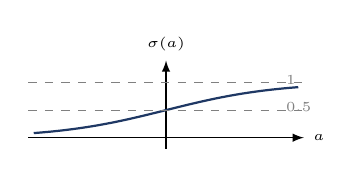
\begin{tikzpicture}[scale=0.7]
        \draw[->] (-2.5,0)--(2.5,0) node[right,font=\tiny]{$a$};
        \draw[->] (0,-0.2)--(0,1.4) node[above,font=\tiny]{$\sigma(a)$};
        \draw[MainBlue,thick,domain=-2.4:2.4,samples=80]
          plot(\x,{1/(1+exp(-\x))});
        \draw[dashed,gray] (-2.5,0.5)--(2.5,0.5);
        \node[right,font=\tiny,gray] at (2.0,0.55) {$0.5$};
        \node[right,font=\tiny,gray] at (2.0,1.05) {$1$};
        \draw[dashed,gray] (-2.5,1)--(2.5,1);
      \end{tikzpicture}
    \end{column}
  \end{columns}
\end{frame}

\begin{frame}{Degrees of Freedom: Discriminative vs.\ Generative}
  \textbf{How many parameters does each approach require?}
  \begin{columns}[T]
    \begin{column}{0.48\textwidth}
      \begin{block}{Logistic Regression}
        \begin{itemize}
          \item Bias $b$ + $d$ weights.
          \item Total: $d+1$ parameters.
        \end{itemize}
      \end{block}
    \end{column}
    \begin{column}{0.48\textwidth}
      \begin{block}{GDA (Gaussian, binary)}
        \begin{itemize}
          \item Two means: $2d$ parameters.
          \item Shared cov.\ matrix: $\frac{d(d+1)}{2}$.
          \item Class prior: $1$ parameter.
          \item Total: $\sim d(d+5)/2 + 1$.
        \end{itemize}
      \end{block}
    \end{column}
  \end{columns}
  \vspace{0.3cm}
  \begin{itemize}
    \item Discriminative models are \mlalert{much more parameter-efficient}.
    \item Preferable in high-dimensional settings or with limited data.
  \end{itemize}
\end{frame}

\begin{frame}{Maximum Likelihood Estimation}
  \textbf{Goal:} estimate $\ow$ from training set $\{(\x_i, t_i)\}_{i=1}^n$.
  \[
    p(t_i|\x_i;\ow) = p_i^{t_i}(1-p_i)^{1-t_i}, \quad p_i = \sigma(\ow^T\ox_i).
  \]
  \textbf{Log-likelihood:}
  \[
    l(\ow|\X,\t) = \sum_{i=1}^n \bigl[t_i\log p_i + (1-t_i)\log(1-p_i)\bigr]
  \]
  \textbf{Gradient:}
  \[
    \nabla_{\ow}\,l(\ow|\X,\t) = \sum_{i=1}^n\bigl(t_i - \sigma(\ow^T\ox_i)\bigr)\ox_i
  \]
  \begin{itemize}
    \item Each sample contributes proportionally to the \emph{prediction error}.
    \item No closed-form solution $\Rightarrow$ iterative optimization.
  \end{itemize}
\end{frame}

\begin{frame}{Gradient Ascent for Logistic Regression}
  \textbf{Update rule} (gradient ascent, step size $\alpha$):
  \[
    \ow^{(j+1)} = \ow^{(j)} + \alpha \sum_{i=1}^n\bigl(t_i - h^{(j)}(\x_i)\bigr)\ox_i
  \]
  \begin{itemize}
    \item Positive error ($t_i > h(\x_i)$): push $\ow$ toward $\ox_i$.
    \item Negative error ($t_i < h(\x_i)$): push $\ow$ away from $\ox_i$.
    \item Same structural form as linear regression updates.
  \end{itemize}
  \vspace{0.3cm}
  \begin{block}{Coordinate-wise update}
    \[
      w_k^{(j+1)} = w_k^{(j)} + \alpha\sum_{i=1}^n\bigl(t_i - \sigma((\w^{(j)})^T\ox_i)\bigr)x_{ik}
    \]
    Update one parameter at a time; same gradient structure.
  \end{block}
\end{frame}

\begin{frame}{Regularization}
  \textbf{Regularized objective:}
  \[
    l_\text{reg}(\ow|\X,\t) = l(\ow|\X,\t) - \frac{\lambda}{2}\|\ow\|^2
  \]
  \begin{columns}[T]
    \begin{column}{0.48\textwidth}
      \begin{block}{$\ell_2$ (Ridge) regularization}
        \begin{itemize}
          \item Adds quadratic penalty.
          \item Gradient: $\nabla l - \lambda\ow$.
          \item Equivalent to Gaussian prior on $\ow$.
          \item Update: $\ow^{(j+1)} = \ow^{(j)} + \alpha[\nabla l - \lambda\ow^{(j)}]$.
          \item Shrinks all weights toward zero.
        \end{itemize}
      \end{block}
    \end{column}
    \begin{column}{0.48\textwidth}
      \begin{block}{$\ell_1$ (Lasso) regularization}
        \begin{itemize}
          \item Adds absolute-value penalty.
          \item Non-differentiable at zero.
          \item Promotes \mlalert{sparsity} in $\ow$.
          \item Equivalent to Laplace prior on $\ow$.
          \item Performs implicit feature selection.
        \end{itemize}
      \end{block}
    \end{column}
  \end{columns}
\end{frame}

%% ── Second-order Methods ──
\subsection{Second-Order Optimization}

\begin{frame}{Newton--Raphson Method (Scalar Case)}
  \textbf{Goal:} find $z$ such that $f(z) = 0$.\\[0.4em]
  \textbf{Update rule:}
  \[
    z_{j+1} = z_j - \frac{f(z_j)}{f'(z_j)}
  \]
  \begin{itemize}
    \item Locally approximates $f$ by its tangent line.
    \item Next iterate: intersection of tangent with the $x$-axis.
  \end{itemize}
  \vspace{0.3cm}
  \textbf{For maximization} (find stationary point of $f$):
  \[
    z_{j+1} = z_j - \frac{f'(z_j)}{f''(z_j)}
  \]
  \begin{itemize}
    \item Curvature $f''(z_j)$ controls step size.
    \item Rapid convergence near a maximum for well-behaved $f$.
  \end{itemize}
\end{frame}

\begin{frame}{Newton--Raphson Method (Multivariate Case)}
  \textbf{Hessian matrix:}
  \[
    \Hmat_{ij}(f) = \frac{\partial^2 f}{\partial w_i \partial w_j}
  \]
  \textbf{Update rule:}
  \[
    \ow^{(j+1)} = \ow^{(j)} - \left.\bigl(\Hmat(f)\bigr)^{-1}\right|_{\ow^{(j)}} \nabla_{\ow}f\big|_{\ow^{(j)}}
  \]
  \begin{itemize}
    \item Inverse Hessian scales the gradient by local curvature.
    \item \mlalert{Faster convergence} than first-order methods.
    \item For linear regression: converges in \emph{one step} (exact quadratic).
  \end{itemize}
  \vspace{0.2cm}
  \begin{block}{For linear regression}
    Gradient: $\nabla E = \oX^T\oX\ow - \oX^T\t$;\quad Hessian: $\Hmat(E) = \oX^T\oX$.\\
    $\Rightarrow\;\ow^{(j+1)} = (\oX^T\oX)^{-1}\oX^T\t$ in one step.
  \end{block}
\end{frame}

\begin{frame}{IRLS: Newton--Raphson for Logistic Regression}
  \textbf{Cross-entropy loss:} $E(\ow) = -l(\ow|\X,\t)$.\\[0.4em]
  \textbf{Gradient and Hessian:}
  \[
    \nabla_{\ow}E = \oX^T(\y - \t), \qquad
    \Hmat(E) = \oX^T\Y\oX
  \]
  where $\Y = \mathrm{diag}(y_i(1-y_i))$ and $y_i = \sigma(\ow^T\ox_i)$.
  \vspace{0.3cm}
  \textbf{Newton--Raphson update:}
  \[
    \ow^{(j+1)} = \ow^{(j)} - \bigl(\oX^T\Y^{(j)}\oX\bigr)^{-1}\oX^T\bigl(\y^{(j)} - \t\bigr)
  \]
  \begin{block}{Weighted least-squares view}
    Introduce \mlalert{adjusted response} $\mathbf{z}^{(j)} = \oX\ow^{(j)} - (\Y^{(j)})^{-1}(\y^{(j)}-\t)$:
    \[
      \ow^{(j+1)} = \bigl(\oX^T\Y^{(j)}\oX\bigr)^{-1}\oX^T\Y^{(j)}\mathbf{z}^{(j)}
    \]
    This is a \mlalert{weighted least squares} problem with weights $\Y^{(j)}$.
  \end{block}
\end{frame}

\begin{frame}{IRLS Algorithm Summary}
  \mlalert{Iteratively Reweighted Least Squares (IRLS):}
  \vspace{0.3cm}
  \begin{enumerate}
    \item Initialize $\ow^{(0)}$ (e.g.\ all zeros).
    \item At each iteration $j$:
      \begin{itemize}
        \item Compute predictions: $y_i = \sigma((\ow^{(j)})^T\ox_i)$.
        \item Compute weight matrix: $\Y^{(j)} = \mathrm{diag}(y_i(1-y_i))$.
        \item Compute adjusted response: $\mathbf{z}^{(j)} = \oX\ow^{(j)} - (\Y^{(j)})^{-1}(\y^{(j)}-\t)$.
        \item Solve: $\ow^{(j+1)} = (\oX^T\Y^{(j)}\oX)^{-1}\oX^T\Y^{(j)}\mathbf{z}^{(j)}$.
      \end{itemize}
    \item Repeat until convergence.
  \end{enumerate}
  \vspace{0.3cm}
  \begin{itemize}
    \item Combines the \emph{fast convergence} of second-order methods.
    \item With the \emph{analytical simplicity} of linear regression.
    \item $\Y^{(j)}$ reflects local slope of the sigmoid at each point.
  \end{itemize}
\end{frame}

%% ── Logistic Regression vs GDA ──
\subsection{Logistic Regression vs.\ GDA}

\begin{frame}{Logistic Regression and Gaussian Discriminant Analysis}
  \textbf{GDA assumption:} $p(\x|C_k) = \mathcal{N}(\x;\Vmu_k,\VSigma)$ (shared covariance).\\[0.4em]
  \begin{itemize}
    \item Applying Bayes' rule gives:
      \[
        \log\frac{p(C_1|\x)}{p(C_2|\x)} = \text{affine function of } \x
        \;\Rightarrow\; p(C_1|\x) = \sigma(\ow^T\ox)
      \]
    \item GDA \mlalert{induces exactly the logistic form} for the posterior.
    \item The converse does \emph{not} hold: logistic regression makes weaker assumptions.
  \end{itemize}
  \vspace{0.3cm}
  \begin{columns}[T]
    \begin{column}{0.48\textwidth}
      \begin{block}{GDA is better when\ldots}
        \begin{itemize}
          \item Data are truly Gaussian.
          \item Training set is small.
        \end{itemize}
      \end{block}
    \end{column}
    \begin{column}{0.48\textwidth}
      \begin{block}{Logistic Reg.\ is better when\ldots}
        \begin{itemize}
          \item Data deviate from normality.
          \item Robustness is preferred.
        \end{itemize}
      \end{block}
    \end{column}
  \end{columns}
\end{frame}

\begin{frame}{Generative vs.\ Discriminative: Key Trade-offs}
  \begin{itemize}
    \item A logistic posterior can arise from many class-conditional distributions (not just Gaussian) — whenever $\log p(\x|C_1)/p(\x|C_2)$ is approximately linear.
    \item GDA \mlalert{uses more structure} (generative model) → effective when assumptions are correct.
    \item Logistic regression \mlalert{uses less structure} → more flexible and robust.
  \end{itemize}
  \vspace{0.3cm}
  \begin{block}{Summary}
    GDA is a more restrictive approach that, when its assumptions hold, yields strong models. Logistic regression sacrifices generative structure in favor of robustness, often providing better predictive performance on complex or partially understood data.
  \end{block}
\end{frame}

%% ══════════════════════════════════════════════════════════════════
\section{Softmax Regression}
%% ══════════════════════════════════════════════════════════════════
%\sectionslide{Softmax Regression}{Multiclass discriminative classification}

\begin{frame}{From Binary to Multiclass}
  \begin{itemize}
    \item Logistic regression handles $K=2$ classes.
    \item For $K > 2$: \mlalert{Softmax Regression} (multinomial logistic regression).
    \item One linear model per class:
      \[
        \overline{\mathbf{W}} = (\w_1, \ldots, \w_K) \in \mathbb{R}^{(d+1)\times K}
      \]
  \end{itemize}
  \vspace{0.3cm}
  \textbf{Class probability via the softmax function:}
  \[
    y_{ik} = p(C_k|\x_i) = \frac{e^{\ow_k^T\ox_i}}{\sum_{r=1}^K e^{\ow_r^T\ox_i}}
  \]
  \begin{itemize}
    \item All probabilities nonneg. and sum to 1.
    \item Classification by argmax of class scores.
    \item Linear decision boundaries between pairs of classes.
  \end{itemize}
\end{frame}

\begin{frame}{Softmax: Training via Maximum Likelihood}
  \textbf{One-hot encoded targets:} $t_{ik} = 1$ if $\x_i \in C_k$, else $0$.\\[0.4em]
  \textbf{Log-likelihood (cross-entropy):}
  \[
    l = \sum_{i=1}^n\sum_{k=1}^K t_{ik}\log y_{ik}
  \]
  \textbf{Gradient per class $k$:}
  \[
    \nabla_{\ow_k}\,l = \sum_{i=1}^n (t_{ik} - y_{ik})\ox_i
  \]
  \begin{itemize}
    \item Structure identical to binary logistic regression.
    \item Each class: \emph{target minus prediction} $\times$ input.
    \item Correctly classified high-confidence points contribute little.
    \item Misclassified/uncertain points drive large updates.
  \end{itemize}
\end{frame}

\begin{frame}{Softmax Regression: Practical Notes}
  \begin{columns}[T]
    \begin{column}{0.55\textwidth}
      \begin{itemize}
        \item Optimization via gradient ascent (batch or stochastic).
        \item Newton--Raphson possible but requires Hessian of size $dK \times dK$ — often too expensive.
        \item First-order methods preferred in large-scale settings.
        \item Cross-entropy objective encourages probability mass on correct classes.
      \end{itemize}
    \end{column}
    \begin{column}{0.42\textwidth}
      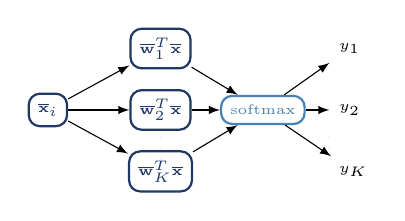
\begin{tikzpicture}[scale=0.65,every node/.style={font=\tiny}]
        \node[draw,MainBlue,thick,rounded corners] (x) at (0,0) {$\ox_i$};
        \node[draw,MainBlue,thick,rounded corners] (s1) at (2.2,1.2) {$\ow_1^T\ox$};
        \node[draw,MainBlue,thick,rounded corners] (s2) at (2.2,0) {$\ow_2^T\ox$};
        \node[draw,MainBlue,thick,rounded corners] (s3) at (2.2,-1.2) {$\ow_K^T\ox$};
        \node[draw,AccentBlue,thick,rounded corners] (sm) at (4.2,0) {softmax};
        \node[right] (y1) at (5.5,1.2) {$y_1$};
        \node[right] (y2) at (5.5,0) {$y_2$};
        \node[right] (y3) at (5.5,-1.2) {$y_K$};
        \draw[->] (x)--(s1); \draw[->] (x)--(s2); \draw[->] (x)--(s3);
        \draw[->] (s1)--(sm); \draw[->] (s2)--(sm); \draw[->] (s3)--(sm);
        \draw[->] (sm)--(y1); \draw[->] (sm)--(y2); \draw[->] (sm)--(y3);
        \node[BlockBg] at (2.2,-0.6) {$\vdots$};
        \node[BlockBg] at (5.5,-0.6) {$\vdots$};
      \end{tikzpicture}
    \end{column}
  \end{columns}
\end{frame}

%% ══════════════════════════════════════════════════════════════════
\section{Probit Regression}
%% ══════════════════════════════════════════════════════════════════
%\sectionslide{Probit Regression}{Alternative activation via stochastic thresholds}

\begin{frame}{Probit Model: Motivation}
  \textbf{General binary GLM:}
  \[
    p(C_1|\x) = f(\w^T\ox)
  \]
  where $f$ maps $\mathbb{R} \to (0,1)$.\\[0.4em]
  \begin{columns}[T]
    \begin{column}{0.55\textwidth}
      \begin{block}{Stochastic threshold model}
        \begin{itemize}
          \item Score: $a = \w^T\ox$.
          \item Random threshold: $\theta \sim \pi(\theta)$.
          \item Classification rule: $\x \in C_1$ iff $a \geq \theta$.
          \item Result: $p(C_1|\x) = \mathbb{P}(\theta \leq a) = \Pi(a)$,\\
                        where $\Pi$ is the CDF of $\pi$.
        \end{itemize}
      \end{block}
    \end{column}
    \begin{column}{0.42\textwidth}
      \begin{itemize}
        \item $\Pi$ must be monotone, bounded between 0 and 1.
        \item Any probability distribution over thresholds gives a valid activation.
        \item Special case: $\pi = \mathcal{N}(0,1) \Rightarrow$ \mlalert{probit} model.
      \end{itemize}
    \end{column}
  \end{columns}
\end{frame}

\begin{frame}{Probit Function}
  \textbf{Standard Gaussian threshold distribution:} $\theta \sim \mathcal{N}(0,1)$.\\[0.3em]
  \textbf{Probit (CDF of standard normal):}
  \[
    \Phi(a) = \int_{-\infty}^a \frac{1}{\sqrt{2\pi}}e^{-\theta^2/2}\,d\theta
  \]
  \textbf{Probit regression:}
  \[
    p(C_1|\x) = \Phi(\w^T\ox)
  \]
  \begin{columns}[T]
    \begin{column}{0.5\textwidth}
      \textbf{Properties of probit:}
      \begin{itemize}
        \item Monotonically increasing.
        \item $0 < \Phi(a) < 1$ for all $a \in \mathbb{R}$.
        \item Smooth S-shaped curve.
        \item Symmetric around 0.
      \end{itemize}
    \end{column}
    \begin{column}{0.46\textwidth}
      \begin{block}{Probit vs.\ sigmoid}
        \begin{itemize}
          \item Qualitatively very similar shapes.
          \item Both give linear decision boundaries.
          \item Probit has heavier tails (slower decay).
          \item Nearly indistinguishable in practice after rescaling.
        \end{itemize}
      \end{block}
    \end{column}
  \end{columns}
\end{frame}

%% ══════════════════════════════════════════════════════════════════
\section{Bayesian Logistic Regression}
%% ══════════════════════════════════════════════════════════════════
%\sectionslide{Bayesian Logistic Regression}{From point estimates to posterior distributions}

\begin{frame}{From MLE to Bayesian Inference}
  \begin{itemize}
    \item MLE / MAP: choose a \emph{single} $\w^*$ and use $p(C_1|\x,\w^*) = \sigma((\w^*)^T\ox)$.
    \item Issues: overfitting, especially with small data, high dimensions, or near-separable classes.
  \end{itemize}
  \vspace{0.3cm}
  \begin{block}{Bayesian approach: posterior predictive}
    \[
      p(C_1|\x,\X,\t) = \int \sigma(\w^T\ox)\,p(\w|\X,\t)\,d\w
    \]
    \begin{itemize}
      \item Predictions average over all plausible $\w$, weighted by the posterior.
      \item Uncertainty in parameters propagates into prediction uncertainty.
      \item More calibrated probabilities; automatic complexity control.
    \end{itemize}
  \end{block}
\end{frame}

\begin{frame}{Posterior Distribution of Coefficients}
  \textbf{Bayes' rule:}
  \[
    p(\w|\X,\t) = \frac{p(\t|\X,\w)\,p(\w)}{p(\t|\X)}
  \]
  \textbf{Likelihood (Bernoulli):}
  \[
    p(\t|\X,\w) = \prod_{i=1}^n \sigma(\w^T\ox_i)^{t_i}\bigl(1-\sigma(\w^T\ox_i)\bigr)^{1-t_i}
  \]
  \begin{itemize}
    \item $p(\t|\X)$ = evidence = normalization constant.
    \item Evidence is key for Bayesian model comparison.
    \item Computing $Z = p(\t|\X)$ in closed form is generally \mlalert{intractable}.
  \end{itemize}
\end{frame}

\begin{frame}{Intractability and Strategies}
  \textbf{Unnormalized posterior:}
  \[
    g(\w;\X,\t) = p(\w)\prod_{i=1}^n \sigma(\w^T\ox_i)^{t_i}(1-\sigma(\w^T\ox_i))^{1-t_i}
  \]
  \begin{itemize}
    \item $g \propto p(\w|\X,\t)$ but we cannot evaluate the normalization $Z$.
    \item Posterior predictive integral is also generally \mlalert{intractable}.
  \end{itemize}
  \vspace{0.2cm}
  \textbf{Standard strategies:}
  \begin{enumerate}
    \item \mlalert{MAP}: find the mode of $p(\w|\X,\t)$ — point estimate.
    \item \mlalert{Variational / Laplace}: approximate $p(\w|\X,\t)$ with a tractable distribution.
    \item \mlalert{Monte Carlo (MCMC)}: sample from $p(\w|\X,\t)$ using only $g(\w;\X,\t)$.
  \end{enumerate}
\end{frame}

%% ── MAP ──
\subsection{MAP Estimation}

\begin{frame}{MAP Estimation for Logistic Regression}
  \textbf{Prior:} $p(\w) = \mathcal{N}(\w|\mathbf{0},\sigma^2\I)$.\\[0.3em]
  \textbf{Log-posterior:}
  \[
    \log p(\w|\X,\t) = -\frac{\w^T\w}{2\sigma^2} + \sum_{i=1}^n\bigl[t_i\log y_i + (1-t_i)\log(1-y_i)\bigr] + c
  \]
  \begin{itemize}
    \item MAP = argmax of log-posterior = maximum of (log-likelihood $-$ $\ell_2$ penalty).
    \item Equivalent to $\ell_2$-regularized logistic regression with $\lambda = 1/\sigma^2$.
    \item Optimization: same Newton--Raphson / IRLS as before, with modified gradient and Hessian.
    \item MAP gives a \emph{single} parameter vector — no uncertainty quantification.
  \end{itemize}
\end{frame}

%% ── Laplace Approximation ──
\subsection{Laplace Approximation}

\begin{frame}{Laplace Approximation: Idea}
  \begin{columns}[T]
    \begin{column}{0.55\textwidth}
      \textbf{Goal:} approximate a distribution $p(\mathbf{z})$ by a Gaussian $q(\mathbf{z}|\Vmu,\VSigma)$ centered at a mode.\\[0.4em]
      \textbf{Motivation:}
      \begin{itemize}
        \item Many posteriors are sharply peaked near their maximum.
        \item A Gaussian provides a good local approximation.
        \item Integrals over a Gaussian are analytically tractable.
      \end{itemize}
    \end{column}
    \begin{column}{0.42\textwidth}
      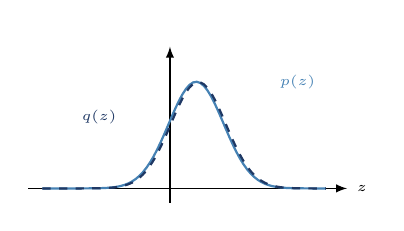
\begin{tikzpicture}[scale=0.9]
        \draw[->] (-2,0)--(2.5,0) node[right,font=\tiny]{$z$};
        \draw[->] (0,-0.2)--(0,2.0) node[above,font=\tiny]{};
        \draw[AccentBlue,thick,domain=-1.8:2.2,samples=80]
          plot(\x,{1.5*exp(-(\x-0.4)^2/0.3)*exp(-0.2*(\x-0.4))});
        \draw[MainBlue,thick,dashed,domain=-1.8:2.2,samples=80]
          plot(\x,{1.5*exp(-(\x-0.4)^2/0.3)});
        \node[AccentBlue,font=\tiny] at (1.8,1.5) {$p(z)$};
        \node[MainBlue,font=\tiny] at (-1.0,1.0) {$q(z)$};
      \end{tikzpicture}
    \end{column}
  \end{columns}
\end{frame}

\begin{frame}{Laplace Approximation: Scalar Case ($d=1$)}
  Let $p(z) = f(z)/Z$, and let $z_0$ be a mode of $f(z)$.\\[0.3em]
  \textbf{Taylor expansion of $\log f(z)$ around $z_0$:}
  \[
    \log f(z) \approx \log f(z_0) - \frac{1}{2}A(z-z_0)^2
  \]
  where $A = -\left.\frac{d^2\log f(z)}{dz^2}\right|_{z=z_0}$ (first derivative vanishes at mode).\\[0.3em]
  \textbf{Gaussian approximation:}
  \[
    q(z) = \frac{\sqrt{A}}{\sqrt{2\pi}}\exp\!\left(-\frac{A}{2}(z-z_0)^2\right)
  \]
  \begin{itemize}
    \item Mean: $\mu = z_0$ (the mode).
    \item Variance: $\sigma^2 = 1/A$ (inverse curvature).
    \item Sharp peaks $\Rightarrow$ small variance $\Rightarrow$ greater certainty.
  \end{itemize}
\end{frame}

\begin{frame}{Laplace Approximation: Multivariate Case ($d>1$)}
  Let $\mathbf{z}_0$ be a mode of $f(\mathbf{z})$.\\[0.3em]
  \textbf{Second-order Taylor expansion:}
  \[
    \log f(\mathbf{z}) \approx \log f(\mathbf{z}_0) - \frac{1}{2}(\mathbf{z}-\mathbf{z}_0)^T\A(\mathbf{z}-\mathbf{z}_0)
  \]
  where $\A = -\left.\frac{\partial^2\log f(\mathbf{z})}{\partial\mathbf{z}^2}\right|_{\mathbf{z}=\mathbf{z}_0}$ is the \mlalert{Hessian of $-\log f$} at the mode.\\[0.4em]
  \textbf{Multivariate Gaussian approximation:}
  \[
    q(\mathbf{z}) = \frac{|\A|^{1/2}}{(2\pi)^{d/2}}\exp\!\left(-\frac{1}{2}(\mathbf{z}-\mathbf{z}_0)^T\A(\mathbf{z}-\mathbf{z}_0)\right)
  \]
  \begin{itemize}
    \item Mean: $\Vmu = \mathbf{z}_0$.
    \item Covariance: $\VSigma = \A^{-1}$.
    \item Strong curvature in a direction $\Rightarrow$ small variance in that direction.
  \end{itemize}
\end{frame}

\begin{frame}{Applying Laplace to Bayesian Logistic Regression}
  \textbf{Gaussian approximation} $q(\w) = \mathcal{N}(\w|\overline{\w},\overline{\VSigma})$:
  \begin{itemize}
    \item $\overline{\w} = \w_{MAP}$ (found via Newton--Raphson / IRLS).
    \item Covariance:
      \[
        \overline{\VSigma} = \left(-\frac{\partial^2}{\partial\w^2}\log p(\w|\X,\t)\right)^{-1}
        = \left(\VSigma_0^{-1} + \sum_{i=1}^n y_i(1-y_i)\ox_i\ox_i^T\right)^{-1}
      \]
    \item Prior precision $\VSigma_0^{-1}$: prevents posterior from being too flat.
    \item Data term: captures informativeness of each observation.
  \end{itemize}
  \vspace{0.2cm}
  \begin{block}{Posterior predictive (still intractable!)}
    \[
      p(C_1|\x,\X,\t) \approx \int \sigma(\w^T\ox)\,\mathcal{N}(\w|\overline{\w},\overline{\VSigma})\,d\w
    \]
    Convolution of sigmoid with Gaussian — no closed form.
  \end{block}
\end{frame}

\begin{frame}{Predictive Distribution: Approximations}
  \textbf{Two routes for the posterior predictive:}
  \vspace{0.3cm}
  \begin{columns}[T]
    \begin{column}{0.48\textwidth}
      \begin{block}{Analytical approximation}
        \[
          p(C_1|\x,\X,\t) \approx \sigma\!\left(\frac{\w_{MAP}^T\ox}{\sqrt{1+\frac{\pi}{8}\ox^T\overline{\VSigma}\ox}}\right)
        \]
        \begin{itemize}
          \item Shrinks the effective margin.
          \item Larger uncertainty $\Rightarrow$ predictions closer to $0.5$.
        \end{itemize}
      \end{block}
    \end{column}
    \begin{column}{0.48\textwidth}
      \begin{block}{Sampling (Monte Carlo)}
        \[
          p(C_1|\x,\X,\t) \approx \frac{1}{N_s}\sum_{i=1}^{N_s}\sigma(\w_i^T\ox)
        \]
        \begin{itemize}
          \item Draw $\w_i \sim \mathcal{N}(\overline{\w},\overline{\VSigma})$.
          \item Average sigmoid over samples.
          \item Simple but requires many samples.
        \end{itemize}
      \end{block}
    \end{column}
  \end{columns}
\end{frame}

%% ── MCMC ──
\subsection{MCMC Sampling}

\begin{frame}{Bayesian Logistic Regression via MCMC}
  \begin{itemize}
    \item Ideal: sample $\w_i$ from the \emph{exact} posterior $p(\w|\X,\t)$.
    \item \mlalert{MCMC}: construct a Markov chain with stationary distribution $= p(\w|\X,\t)$.
    \item After burn-in, chain states are (dependent) samples from the posterior.
  \end{itemize}
  \vspace{0.3cm}
  \textbf{Predictive distribution:}
  \[
    p(C_1|\x,\X,\t) \approx \frac{1}{N_s}\sum_{i=1}^{N_s}\sigma(\w_i^T\ox), \quad \w_i \sim p(\w|\X,\t)
  \]
  \begin{columns}[T]
    \begin{column}{0.48\textwidth}
      \begin{block}{Advantages}
        \begin{itemize}
          \item No restrictive parametric approximation.
          \item Approximates true Bayesian averaging.
        \end{itemize}
      \end{block}
    \end{column}
    \begin{column}{0.48\textwidth}
      \begin{block}{Disadvantages}
        \begin{itemize}
          \item Computationally expensive.
          \item Careful tuning of chain needed.
          \item Correlated samples require many iterations.
        \end{itemize}
      \end{block}
    \end{column}
  \end{columns}
\end{frame}

\begin{frame}{MCMC Algorithms}
  \textbf{Classical methods:}
  \begin{itemize}
    \item \mlalert{Metropolis--Hastings}: proposes new states and accepts/rejects stochastically.
    \item \mlalert{Gibbs Sampling}: updates one parameter at a time from its conditional distribution.
  \end{itemize}
  \vspace{0.3cm}
  \textbf{Advanced methods:}
  \begin{itemize}
    \item Exploit gradient information (Langevin, Hamiltonian Monte Carlo).
    \item Improve efficiency in high-dimensional parameter spaces.
    \item Essential principle: construct a chain that mixes well and converges to the correct stationary distribution.
  \end{itemize}
  \vspace{0.2cm}
  \begin{block}{Key insight}
    MCMC provides Bayesian averaging without requiring closed-form normalization constants — at the cost of computation.
  \end{block}
\end{frame}

%% ══════════════════════════════════════════════════════════════════
\section{Summary}
%% ══════════════════════════════════════════════════════════════════
%\sectionslide{Summary}{Key concepts and connections}

\begin{frame}{Chapter Summary: GLMs and Classification}
  \begin{columns}[T]
    \begin{column}{0.48\textwidth}
      \textbf{Generalized Linear Models:}
      \begin{itemize}
        \item Unifying framework: linear predictor + nonlinear response.
        \item Response function determined by exponential family.
        \item Always yields linear decision boundaries.
        \item Includes: linear regression, logistic, softmax, Poisson regression.
      \end{itemize}
    \end{column}
    \begin{column}{0.48\textwidth}
      \textbf{Discriminative Classification:}
      \begin{itemize}
        \item Model $p(C_k|\x)$ directly.
        \item Fewer parameters than generative models.
        \item More robust to distributional misspecification.
        \item Logistic regression: canonical binary classifier.
        \item Softmax regression: canonical multiclass classifier.
      \end{itemize}
    \end{column}
  \end{columns}
\end{frame}

\begin{frame}{Chapter Summary: Optimization and Bayesian Inference}
  \begin{columns}[T]
    \begin{column}{0.48\textwidth}
      \textbf{Optimization:}
      \begin{itemize}
        \item First-order: gradient ascent (simple, robust).
        \item Second-order: Newton--Raphson / IRLS (fast convergence).
        \item IRLS = weighted least squares at each step.
        \item Regularization ($\ell_1$/$\ell_2$) for overfitting control.
      \end{itemize}
    \end{column}
    \begin{column}{0.48\textwidth}
      \textbf{Bayesian Logistic Regression:}
      \begin{itemize}
        \item Posterior $p(\w|\X,\t)$ is intractable.
        \item MAP: simplest, point estimate.
        \item Laplace: Gaussian approximation at the mode.
        \item MCMC: most accurate, most expensive.
        \item Bayesian averaging $\Rightarrow$ better calibration.
      \end{itemize}
    \end{column}
  \end{columns}
\end{frame}

%\begin{frame}{Connection Map}
%  \begin{center}
%  \begin{tikzpicture}[
%    box/.style={draw,rounded corners,fill=MainBlue!15,font=\small,inner sep=6pt,text width=2.5cm,align=center},
%    arrow/.style={-{Stealth},MainBlue,thick},
%    darrow/.style={-{Stealth},AccentBlue,thick,dashed},
%    scale=0.9
%  ]
%    \node[box] (expfam) at (0,3) {Exponential Family};
%    \node[box] (glm) at (4,3) {GLM Framework};
%    \node[box] (lr) at (2,1.5) {Logistic Regression};
%    \node[box] (sr) at (6,1.5) {Softmax Regression};
%    \node[box] (irls) at (2,0) {IRLS Optimization};
%    \node[box] (bayes) at (6,0) {Bayesian Inference};
%    \draw[arrow] (expfam)--(glm);
%    \draw[arrow] (glm)--(lr);
%    \draw[arrow] (glm)--(sr);
%    \draw[arrow] (lr)--(irls);
%    \draw[darrow] (lr)--(bayes);
%    \node[font=\tiny,BlockBg] at (4,2.6) {+linear predictor};
%  \end{tikzpicture}
%  \end{center}
%\end{frame}

%\end{document}
